\section{Method}

In order to lay the foundation for the ISA task, we propose a novel baseline method to perform the task.
% called \textbf{V}ision-\textbf{L}anguage collaborative \textbf{ISA} method (\textbf{VLISA}) 
Since we expect to assess images from a higher semantic level, and language can usually express semantics more directly than images, we believe hybrid utilization of both visual and language information will be helpful for ISA task. 
Thus, we propose the \textbf{V}ision-\textbf{L}anguage collaborative \textbf{ISA} (\textbf{VLISA}) method.

% \MY{say something that extracting semantics information from an image requires hybrid utilization of visual and language information, therefore we propose a xxxx}

\begin{figure}[H]
    \centering
    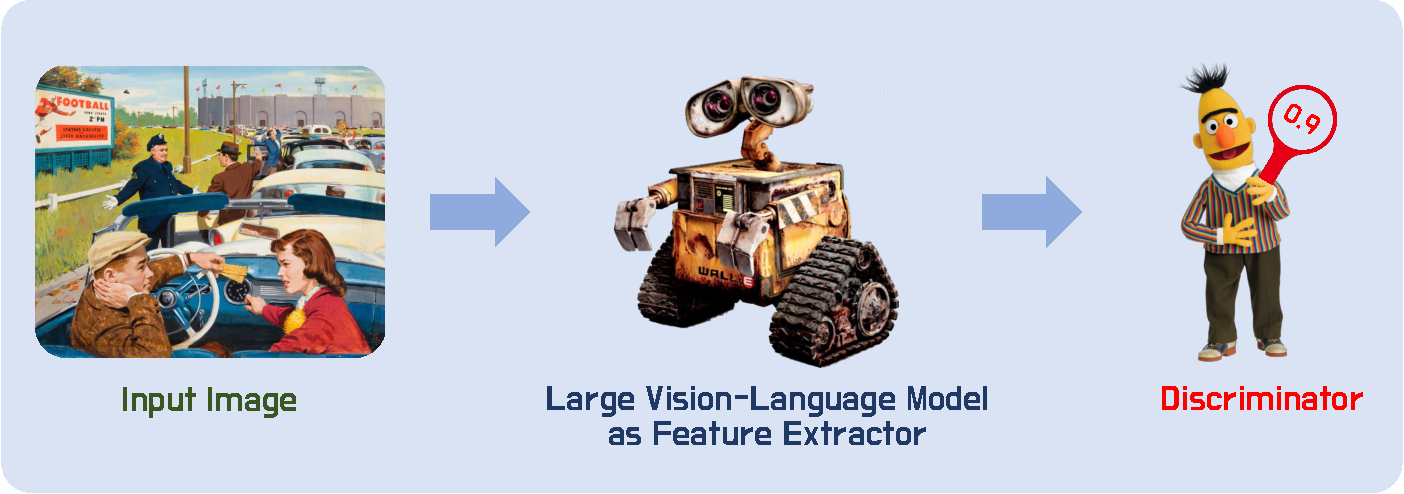
\includegraphics[scale=0.33]{figs/pipeline2.pdf}
    \caption{Pipeline of our proposed VLISA method. }
    \label{method}
\end{figure}

As shown in Figure~\ref{method}, VLISA has two components: a Feature Extractor and a Discriminator.
This design follows the typical flow of IAA systems, which consists of a Feature Extraction phase and a Decision Phase~\cite{deng2017image}.
Specifically, we first use a LVLM as the Feature Extractor to extract semantic information in natural language form as features from images.
We adopt GPT-4o~\cite{gpt4} in this paper, considering its strong Vision-Language capability.
Then, we use a Discriminator model, such as BERT~\cite{devlin-etal-2019-bert}, to rate the input image based on the extracted features.
One advantage of using LVLM as the Feature Extractor is that it can mitigate the impact of different image styles and types and focus more on semantics in images.
According to different feature extraction modes, we propose two versions of VLISA.

\paragraph{Naive VLISA}

The first way for GPT-4o to extract features from the input image is to make it describe the image in detail.
The prompt is simple as: 
\texttt{Describe this image in detail.} 
The generated description is later taken as the input of the Discriminator model.
% \MY{Such information is later taken as the input xxxx}

\paragraph{Chain-of-Thought VLISA}  % Reasoning

The second feature extraction method is inspired by Chain-of-Thought (CoT)~\cite{cot2024}. 
Referring to the annotation instruction of CogBench~\cite{song2024cognitive}, we first ask GPT-4o to generate Chain-of-Reasonings (CoRs) from different aspects, then generate the description based on the CoRs. 
A CoR consists of visual clues and the conclusion drawn from the clues.

Specifically, we adopt seven categories of CoRs:  %visual clues: 
% [Special Time], [Special Location], [Character Role], [Character Relationship], [High-level Event], [Event Causal Relationship], and [Mental State].

\begin{itemize}
    \item \textbf{Special Time.} ``Special time'' refers to a time that requires observation of clues to deduce, rather than an obvious time like ``daytime.''
    \item \textbf{Special Location.} ``Special location'' refers to a location that requires observation of clues to deduce, rather than an obvious location like ``on the roadside.''
    \item \textbf{Character Role.} The roles or identities of characters in the images.
    \item \textbf{Character Relationship.} The relationships between characters in the images.
    \item \textbf{High-level Event.} ``High-level events'' refer to events that require observation of clues to deduce, rather than obvious actions like ``running.''
    \item \textbf{Event Causal Relationship.} The causal relationships between events in the images.
    \item \textbf{Mental State.} Mental states of characters (or animals) in the images.
\end{itemize}

The detailed prompt is shown in Technical Appendix.

% The detailed prompt is shown in Figure~\ref{cot_prompt}.

Both the generated CoRs and description are later used as input for the Discriminator model.